\PassOptionsToPackage{unicode=true}{hyperref} % options for packages loaded elsewhere
\PassOptionsToPackage{hyphens}{url}
%
\documentclass[]{article}
\usepackage{lmodern}
\usepackage{amssymb,amsmath}
\usepackage{ifxetex,ifluatex}
\usepackage{fixltx2e} % provides \textsubscript
\ifnum 0\ifxetex 1\fi\ifluatex 1\fi=0 % if pdftex
  \usepackage[T1]{fontenc}
  \usepackage[utf8]{inputenc}
  \usepackage{textcomp} % provides euro and other symbols
\else % if luatex or xelatex
  \usepackage{unicode-math}
  \defaultfontfeatures{Ligatures=TeX,Scale=MatchLowercase}
    \setmainfont[]{cantarell}
\fi
% use upquote if available, for straight quotes in verbatim environments
\IfFileExists{upquote.sty}{\usepackage{upquote}}{}
% use microtype if available
\IfFileExists{microtype.sty}{%
\usepackage[]{microtype}
\UseMicrotypeSet[protrusion]{basicmath} % disable protrusion for tt fonts
}{}
\IfFileExists{parskip.sty}{%
\usepackage{parskip}
}{% else
\setlength{\parindent}{0pt}
\setlength{\parskip}{6pt plus 2pt minus 1pt}
}
\usepackage{hyperref}
\hypersetup{
            pdftitle={WizMe},
            pdfborder={0 0 0},
            breaklinks=true}
\urlstyle{same}  % don't use monospace font for urls
\usepackage[margin=2cm]{geometry}
\usepackage{longtable,booktabs}
% Fix footnotes in tables (requires footnote package)
\IfFileExists{footnote.sty}{\usepackage{footnote}\makesavenoteenv{longtable}}{}
\usepackage{graphicx,grffile}
\makeatletter
\def\maxwidth{\ifdim\Gin@nat@width>\linewidth\linewidth\else\Gin@nat@width\fi}
\def\maxheight{\ifdim\Gin@nat@height>\textheight\textheight\else\Gin@nat@height\fi}
\makeatother
% Scale images if necessary, so that they will not overflow the page
% margins by default, and it is still possible to overwrite the defaults
% using explicit options in \includegraphics[width, height, ...]{}
\setkeys{Gin}{width=\maxwidth,height=\maxheight,keepaspectratio}
\setlength{\emergencystretch}{3em}  % prevent overfull lines
\providecommand{\tightlist}{%
  \setlength{\itemsep}{0pt}\setlength{\parskip}{0pt}}
\setcounter{secnumdepth}{3}
% Redefines (sub)paragraphs to behave more like sections
\ifx\paragraph\undefined\else
\let\oldparagraph\paragraph
\renewcommand{\paragraph}[1]{\oldparagraph{#1}\mbox{}}
\fi
\ifx\subparagraph\undefined\else
\let\oldsubparagraph\subparagraph
\renewcommand{\subparagraph}[1]{\oldsubparagraph{#1}\mbox{}}
\fi

% set default figure placement to htbp
\makeatletter
\def\fps@figure{htbp}
\makeatother

\makeatletter
\@ifpackageloaded{subfig}{}{\usepackage{subfig}}
\@ifpackageloaded{caption}{}{\usepackage{caption}}
\captionsetup[subfloat]{margin=0.5em}
\AtBeginDocument{%
\renewcommand*\figurename{Figure}
\renewcommand*\tablename{Table}
}
\AtBeginDocument{%
\renewcommand*\listfigurename{List of Figures}
\renewcommand*\listtablename{List of Tables}
}
\@ifpackageloaded{float}{}{\usepackage{float}}
\floatstyle{ruled}
\@ifundefined{c@chapter}{\newfloat{codelisting}{h}{lop}}{\newfloat{codelisting}{h}{lop}[chapter]}
\floatname{codelisting}{Listing}
\newcommand*\listoflistings{\listof{codelisting}{List of Listings}}
\makeatother

\title{WizMe}
\date{}

\begin{document}
\maketitle

\href{https://ec.europa.eu/info/funding-tenders/opportunities/portal/screen/opportunities/topic-details/fetopen-01-2018-2019-2020;freeTextSearchKeyword=;typeCodes=1;statusCodes=31094501,31094502;programCode=null;programDivisionCode=null;focusAreaCode=null;crossCuttingPriorityCode=null;callCode=31088571;sortQuery=openingDate;onlyTenders=false}{\textbf{FET
Open} call details on EU website}

\hypertarget{title-of-the-proposal}{%
\subsection{Title of the proposal}\label{title-of-the-proposal}}

\textbf{Social robots to support human-human interactions}

\hypertarget{acronym}{%
\subsection{Acronym}\label{acronym}}

WizMe

\hypertarget{consortium}{%
\subsection{Consortium}\label{consortium}}

\begin{itemize}
\tightlist
\item
  Bristol Robotics Lab (BRL), \emph{Séverin Lemaignan, Manuel Giuliani}
\item
  Univeristy of Ghent (GHE), \emph{Tony Belpaeme, Jelle Saldien}
\item
  École Polytechnique Fédérale de Lausanne (EPFL), \emph{Pierre
  Dillenbourg} (tentative)
\item
  Instituto Superior Técnico, University of Lisbon (IST), \emph{Ana
  Paiva} (tentative)
\item
  Academic partner in sociology -- Radboud University Nijmegen?
\item
  RedCross UK (RCUK), \emph{Alex Fraser} (first contact; tentative)
\end{itemize}

\hypertarget{abstract}{%
\subsection{Abstract}\label{abstract}}

WizMe is a future-looking project that aims at investigating how social
robots can help building stronger \emph{human} relationships: robots to
support human-human social interactions.

Such robots require unique, beyond state-of-the-art, capabilities to
\emph{(1)} understand the social interactions (\emph{social situation
awareness}), \emph{(2)} decide the best course of action for short-term
and longer-term social influence, and \emph{(3)} perform the appropriate
social acts.

In the WizMe project, we propose to scaffold this radically novel line
of research with an original application of high societal impact: we
will create a small set of novel personal companion robots designed to
facilitate human-human interactions. These robots will be deployed in
selected school to support the social and cultural integration of
vulnerable children, with a particular focus on migrant children who
might lack the otherwise needed support for a successful integration
(different cultures and social norms; absence of local, culturally
integrated, relatives; language barriers; etc.).

This project is ambitious, and brings together five leading groups in
social human-robot interaction, interaction design and human
socio-developmental psychology, with unique expertise and contributions:
The Bristol Robotics Lab, the largest UK robotic lab, has a long history
of running and leading complex projects involving hardware, software and
AI, with a strong track record in human-robot interaction and assistive
robotics; the University of Ghent will provide world-leading expertise
on robot design for interaction with children; the EPFL's CHILI lab has
a unique expertise in blending technology (and social robotics in
particular) in teaching environments, with a focus on rich social
interaction; the IST is recognised as a leading group in expressive
social agents and also has a very strong track record in child-robot
interactions; finally {[}socio-psychology partner{]}.

Critically, the complex interaction design that lies at the core of the
project will be informed and co-led by the Refugee Support department of
RedCross UK, one of the largest NGO world-wide.

\pagebreak

\textbf{{[}Sections 1, 2, 3 are 15 pages max{]}}

\hypertarget{excellence}{%
\section{Excellence}\label{excellence}}

\hypertarget{long-term-vision-and-targeted-breakthrough-towards-that-vision}{%
\subsection{Long-term vision and targeted breakthrough towards that
vision}\label{long-term-vision-and-targeted-breakthrough-towards-that-vision}}

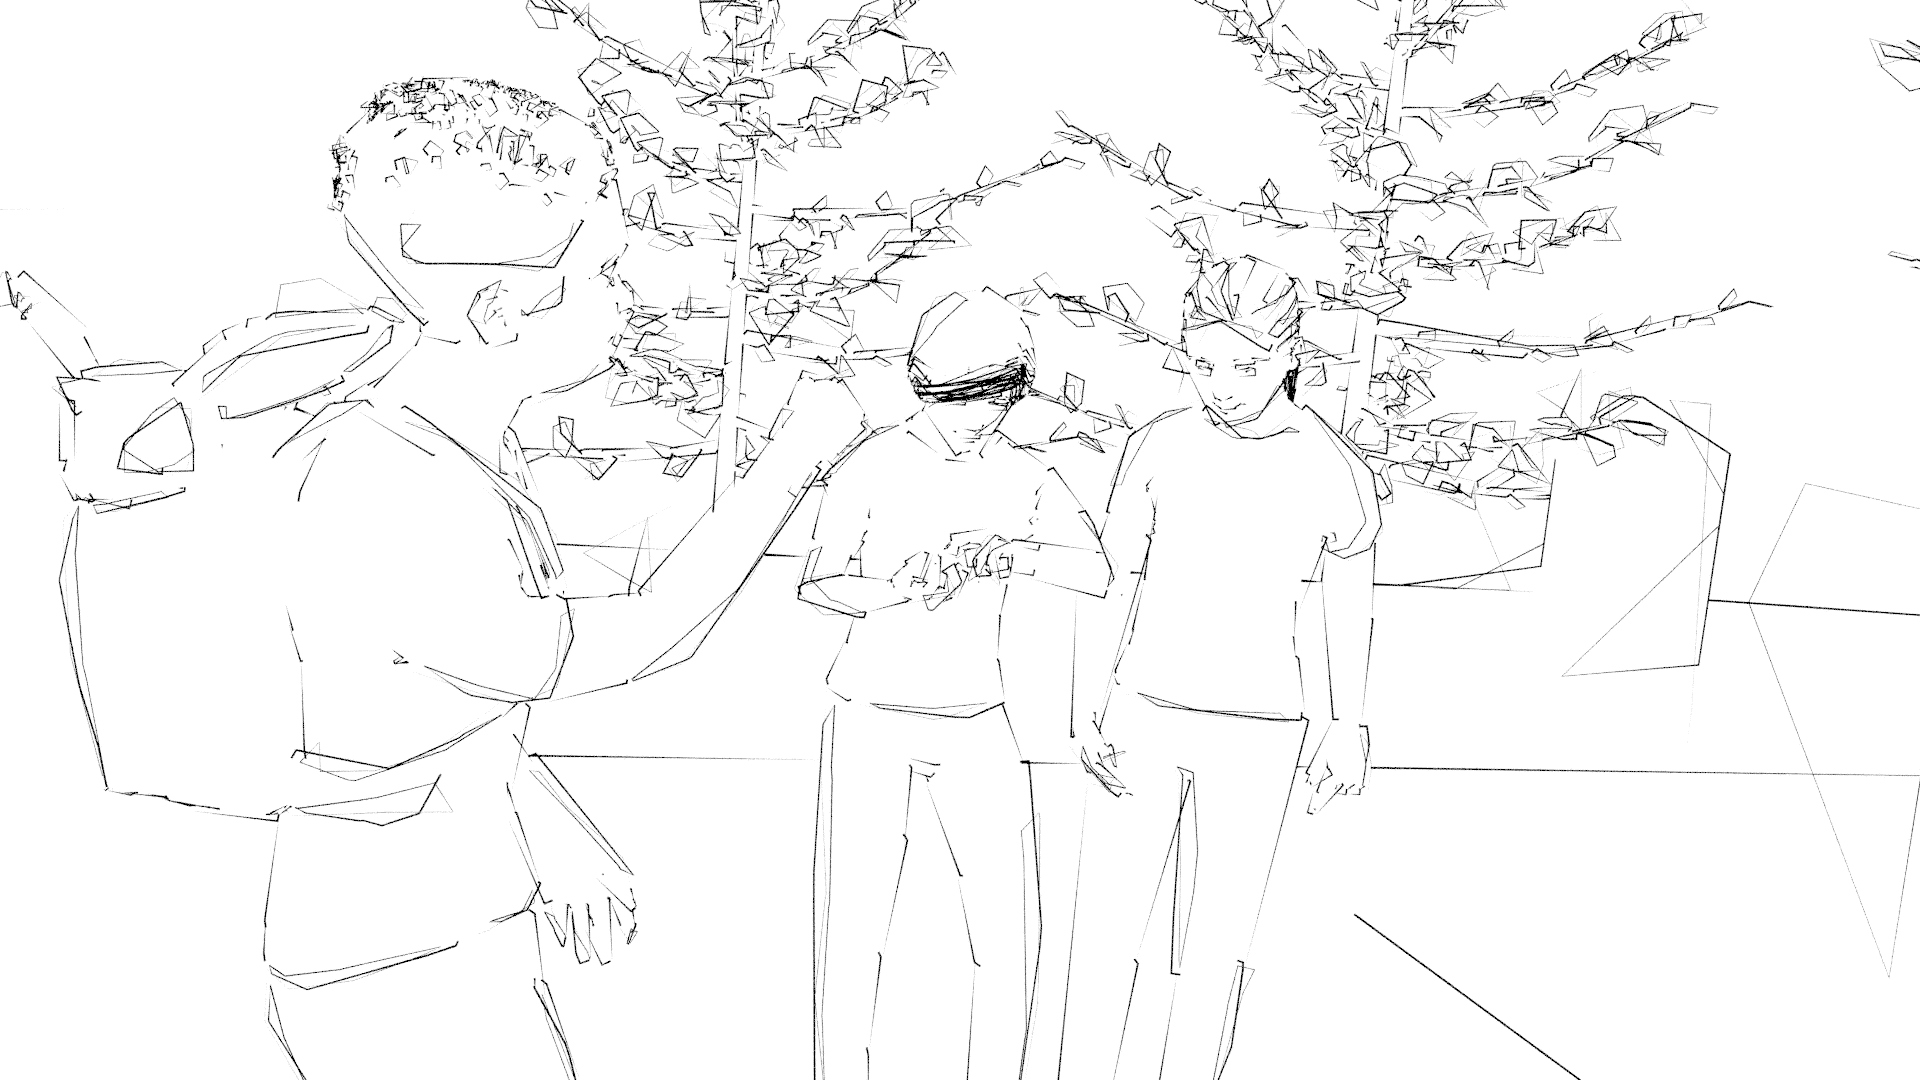
\includegraphics{figs/render5.png}~

WizMe is a project that aims at helping to build strong human
relationships with the help of technology.

The core idea of the project is to build small companion robots whose
aim is to facilitate human-human interactions. We want to develop these
robots with a particular application in mind: supporting the social and
cultural integration of vulnerable children in a foreign country, and in
particular, migrant children who might lack the otherwise needed support
(shared culture; already well integrated relatives) for a successful
integration.

\hypertarget{key-scientific-research-questions}{%
\subsubsection{Key scientific research
questions}\label{key-scientific-research-questions}}

\begin{itemize}
\tightlist
\item
  explore the novel concept of robot-supported human-human interactions:
\item
  establish trust between the child and the robot
\item
  mediation of cross-cultural interactions
\item
  modalities of interactions that are well suited for the field
\item
  privacy
\item
  \ldots{}
\end{itemize}

\hypertarget{novelty-non-incrementality-plausibility-and-foundational-character}{%
\subsection{Novelty, non-incrementality, plausibility and foundational
character}\label{novelty-non-incrementality-plausibility-and-foundational-character}}

\hypertarget{existing-robots}{%
\paragraph{Existing robots}\label{existing-robots}}

\hypertarget{miro}{%
\subparagraph{Miro}\label{miro}}

\begin{figure}
\centering
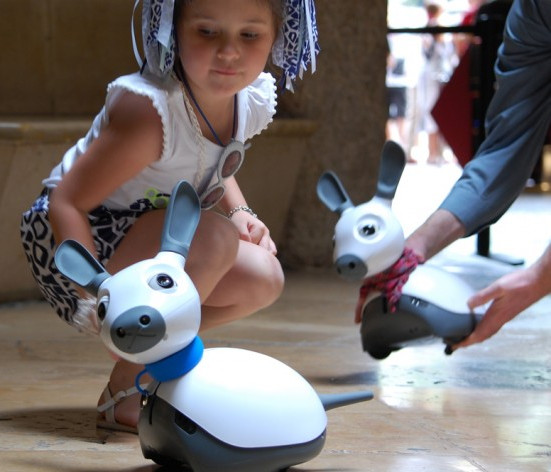
\includegraphics[width=0.5\textwidth,height=\textheight]{figs/miro.jpg}
\caption{Consequential Miro robot}
\end{figure}

\begin{figure}
\centering
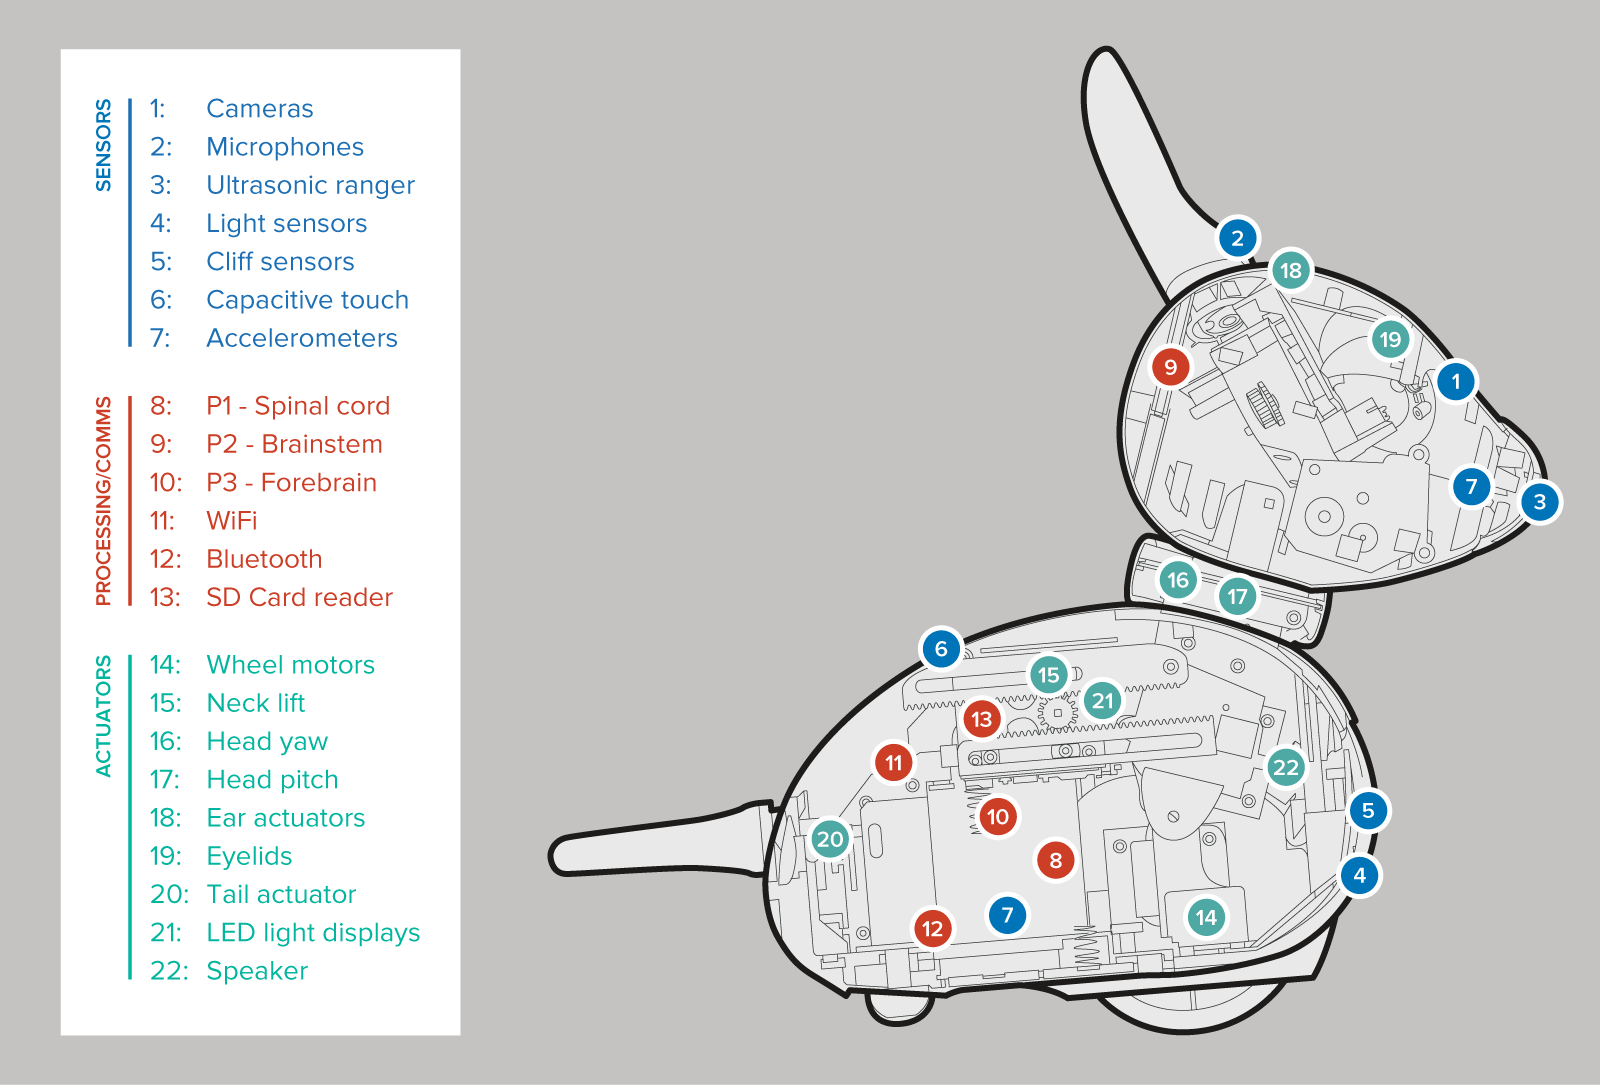
\includegraphics[width=0.5\textwidth,height=\textheight]{figs/miro-spec.png}
\caption{Consequential Miro specifications}
\end{figure}

\hypertarget{hatchnimals}{%
\subparagraph{Hatchnimals}\label{hatchnimals}}

\begin{figure}
\centering
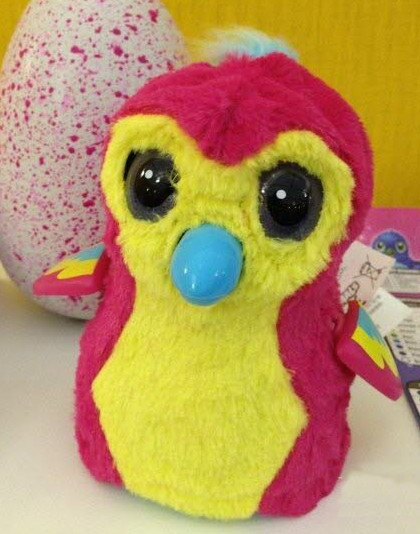
\includegraphics[width=0.5\textwidth,height=\textheight]{figs/hatchnimals.jpg}
\caption{Hatchnimals}
\end{figure}

\hypertarget{tega}{%
\subparagraph{Tega}\label{tega}}

\begin{figure}
\centering
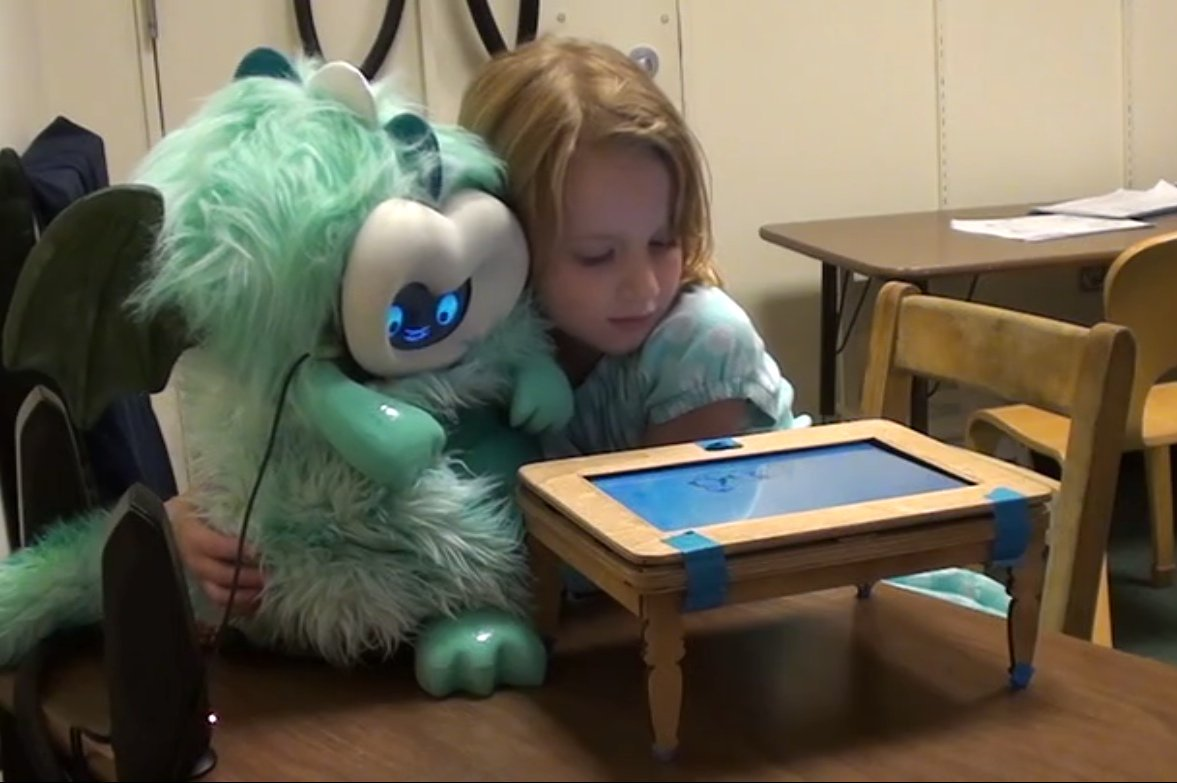
\includegraphics[width=0.5\textwidth,height=\textheight]{figs/tega.jpg}
\caption{MediaLab's Tega robot}
\end{figure}

\hypertarget{cellulo}{%
\subparagraph{Cellulo}\label{cellulo}}

\begin{figure}
\centering
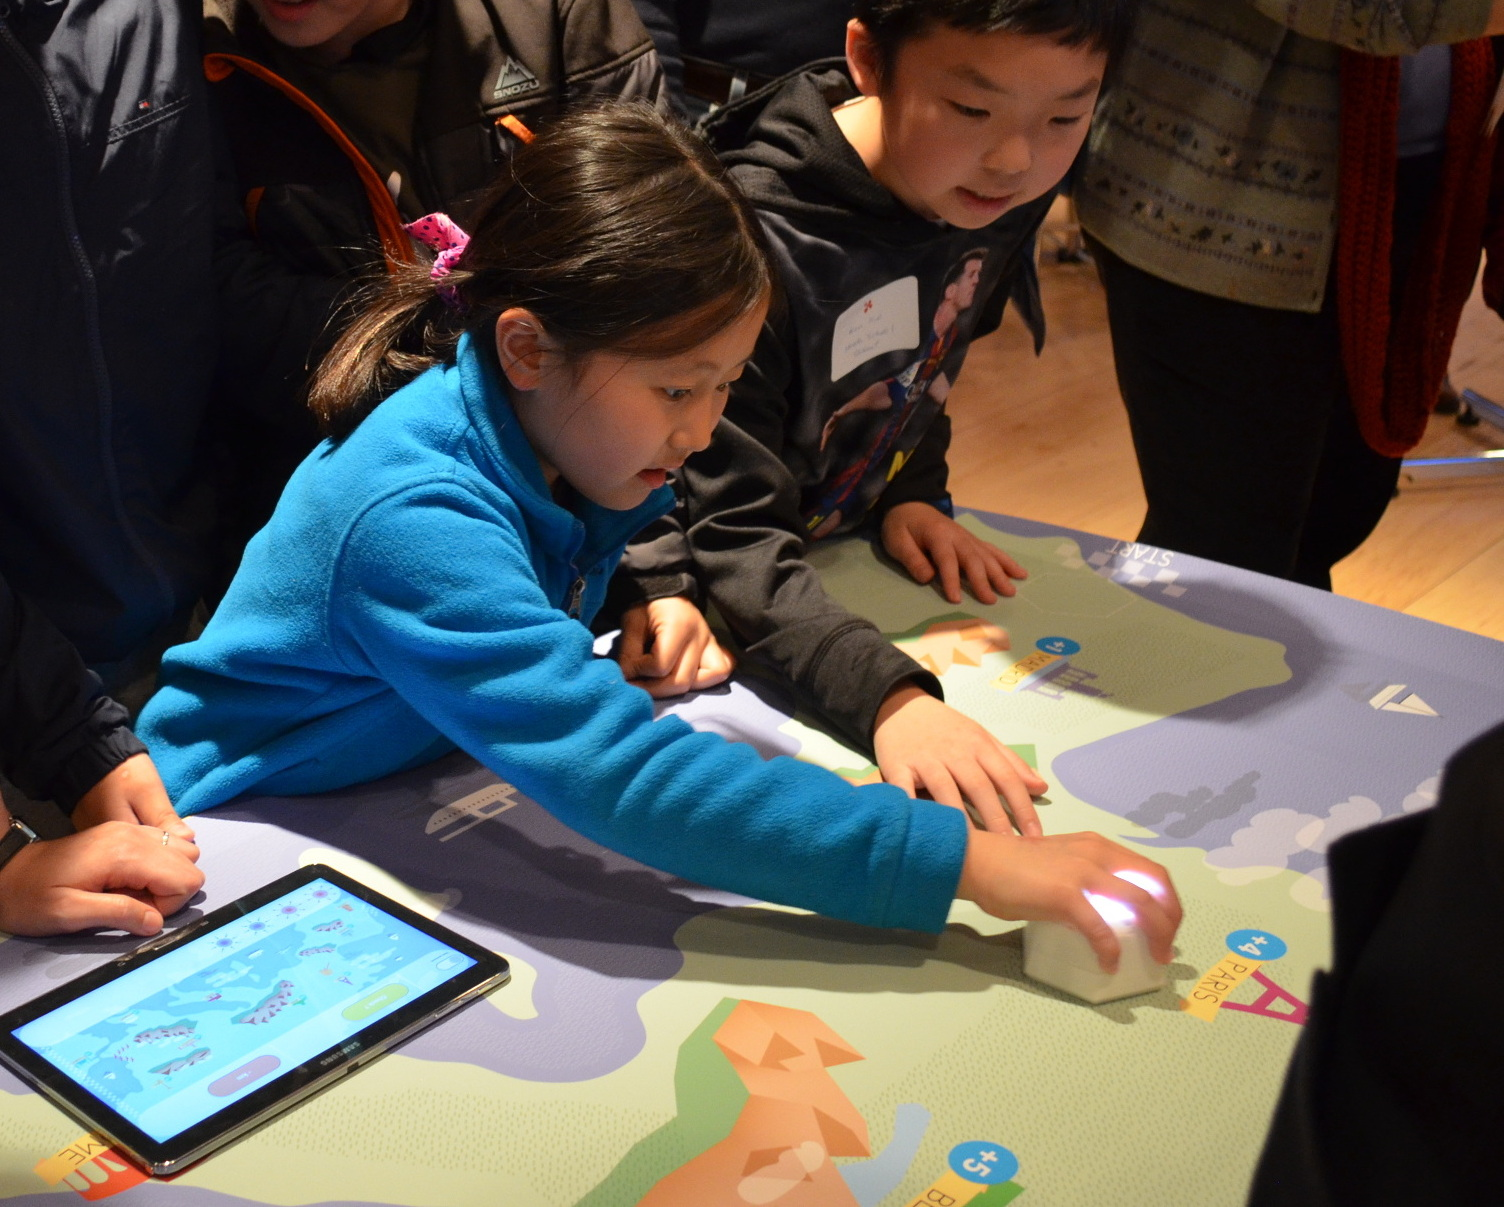
\includegraphics[width=0.5\textwidth,height=\textheight]{figs/cellulo.jpg}
\caption{EPFL's Cellulo robot}
\end{figure}

(Özgür et al. 2017)

\hypertarget{cozmo}{%
\subparagraph{Cozmo}\label{cozmo}}

\begin{figure}
\centering
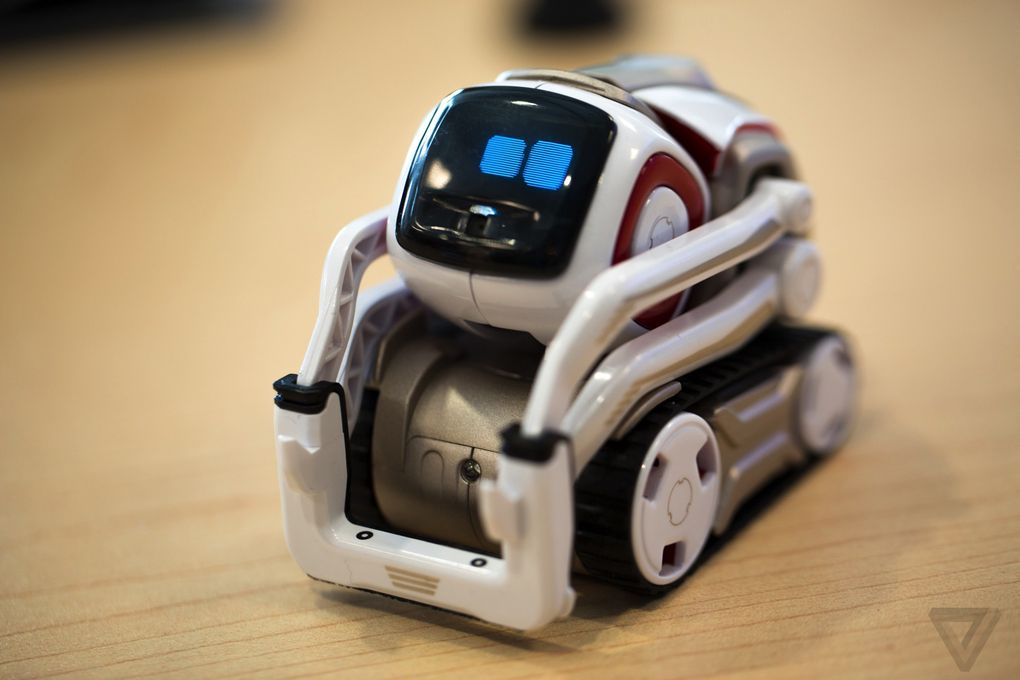
\includegraphics[width=0.5\textwidth,height=\textheight]{figs/anki-cozmo.jpg}
\caption{Anki's Cozmo}
\end{figure}

\begin{figure}
\centering
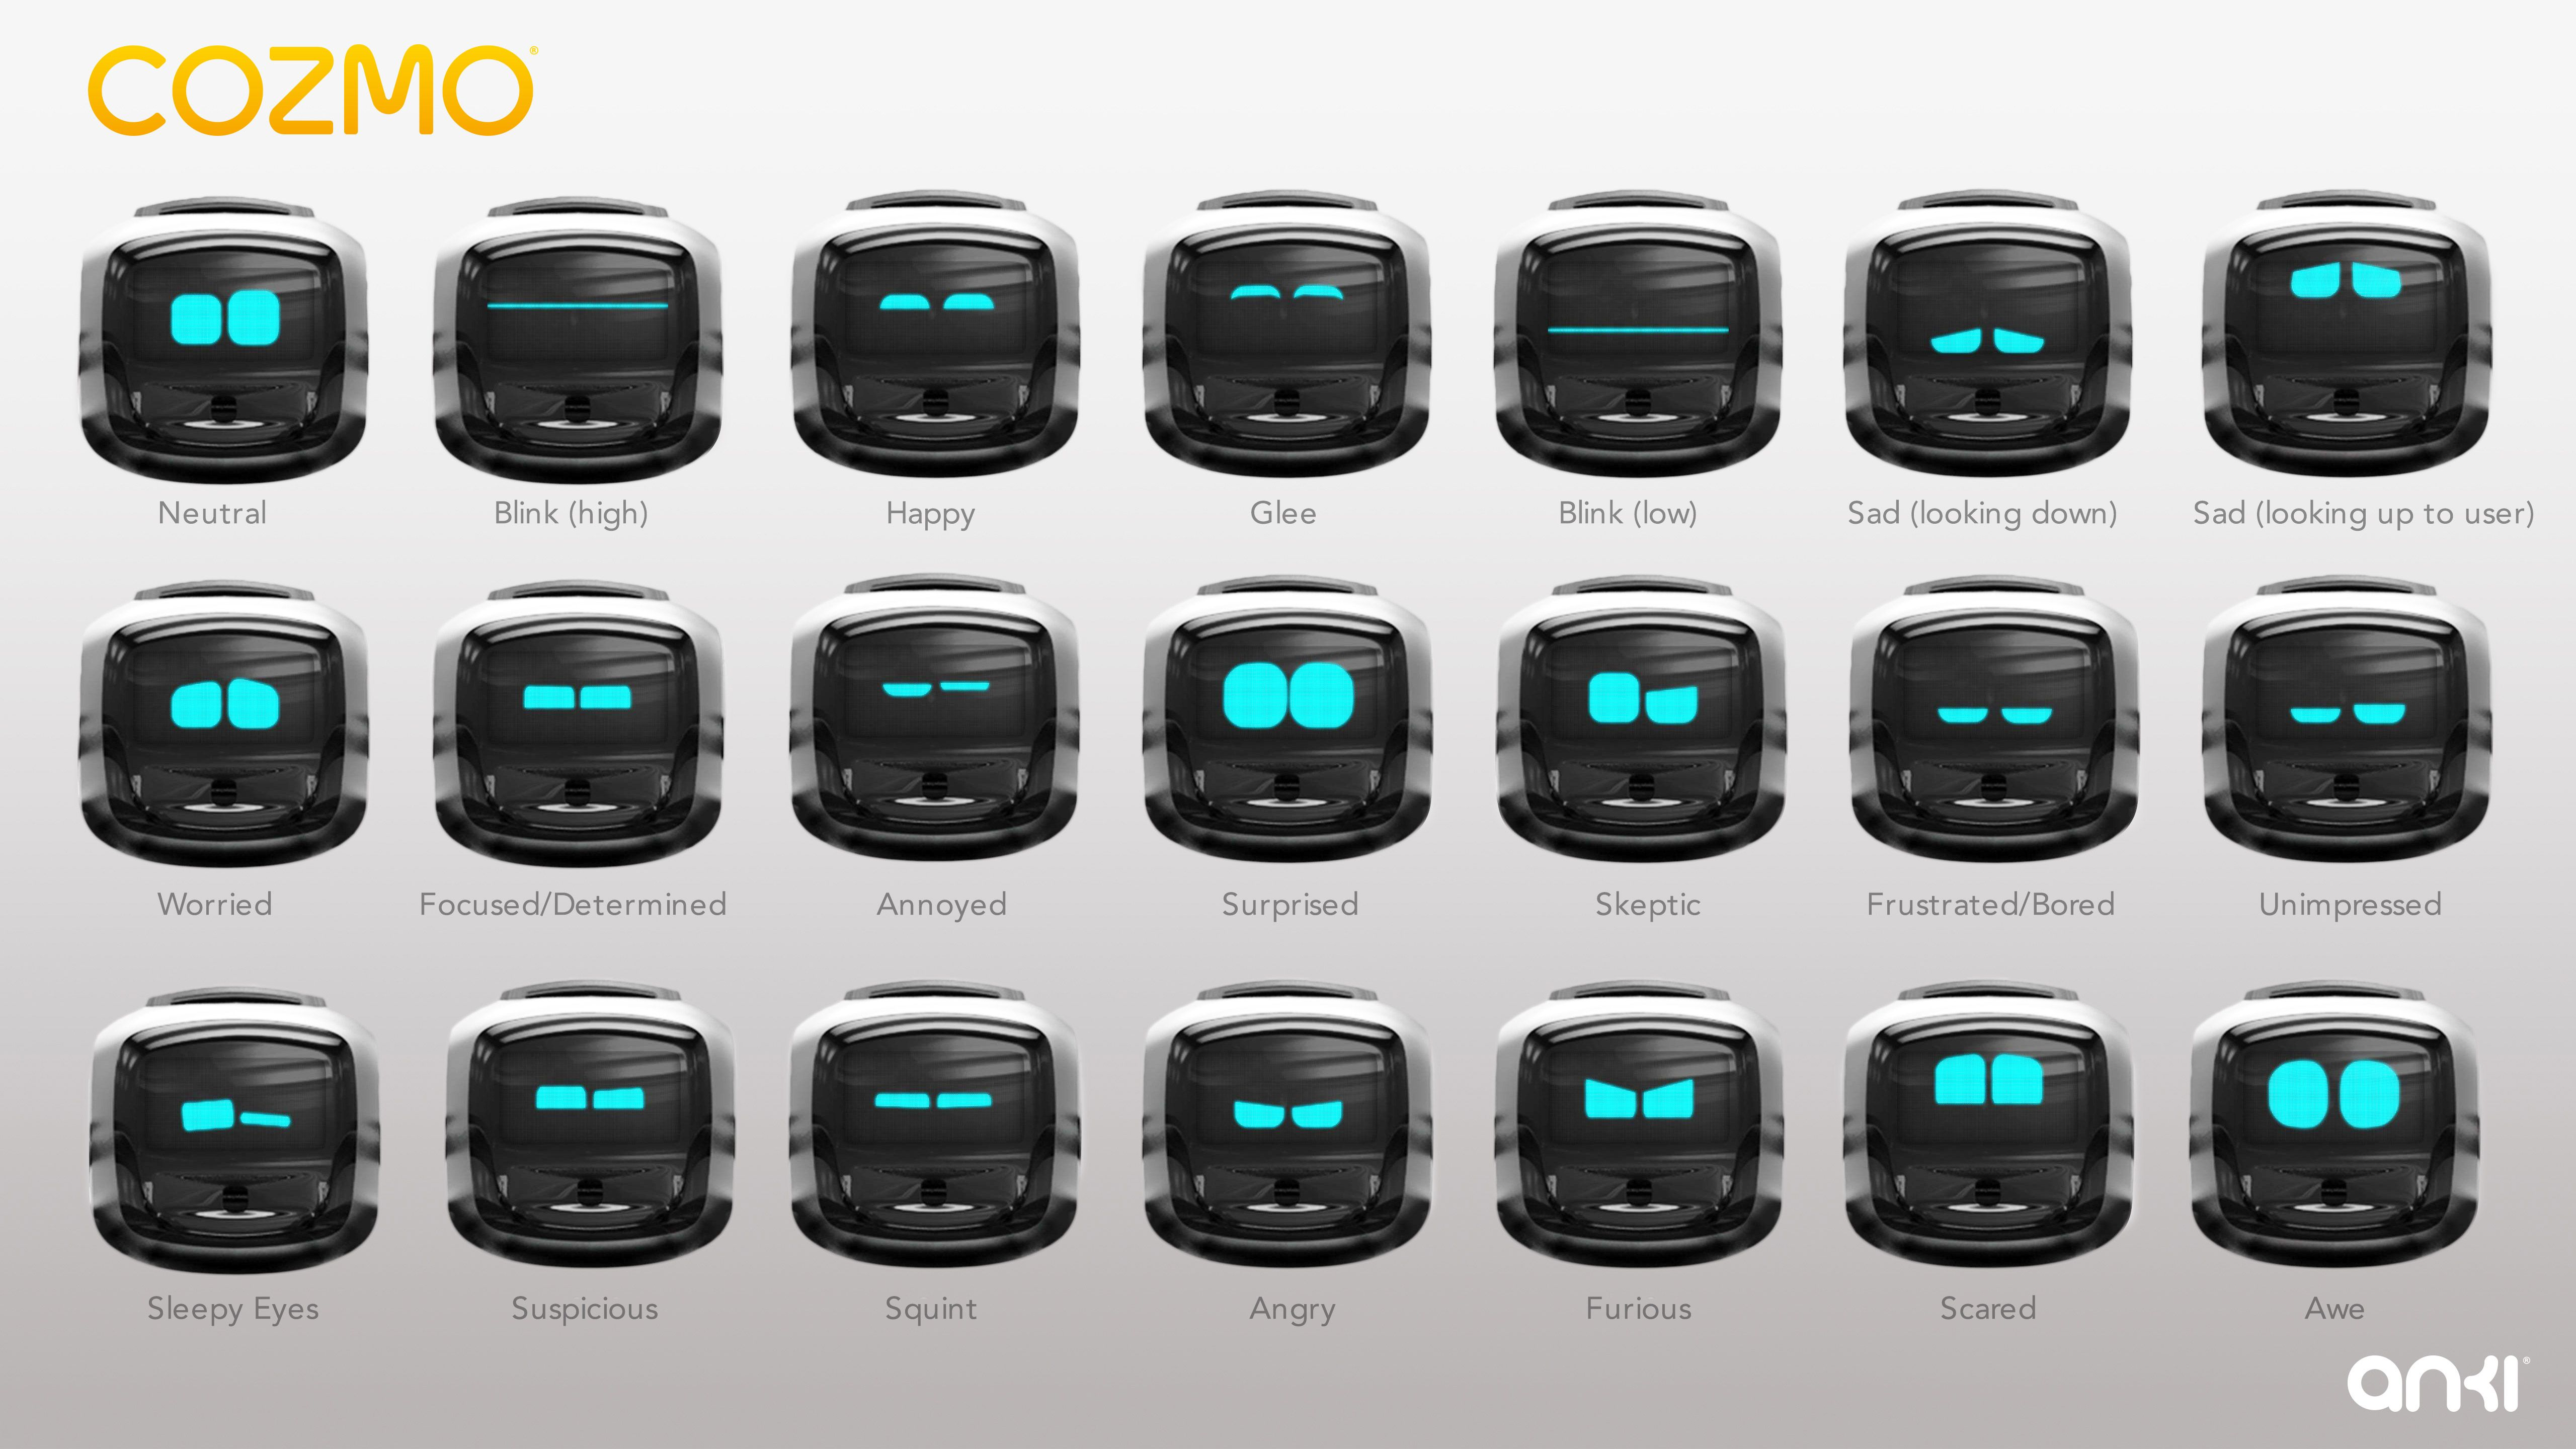
\includegraphics{figs/cozmo-expression-sheet.jpg}
\caption{Cozmo facial expressions}
\end{figure}

\hypertarget{research-methodology}{%
\subsection{Research methodology}\label{research-methodology}}

\hypertarget{overview-of-the-interaction}{%
\subsubsection{Overview of the
interaction}\label{overview-of-the-interaction}}

A robot is left with the child when he or she starts their journey in
their new host country, and becomes a companion for the child during the
first months of the integration. Using several mechanisms that are
discussed in this proposal, the robot helps the child to gain
self-confidence, and ultimately engage in successful social interactions
with other children.

Critically, the robot is designed to support the social and cultural
integration of the child \emph{amongst her/his peers}. While the child
might build affective/emotional bonds with the robot over the course of
the support period, the robot behaviour is designed to ensure that these
bonds do not substitute themselves to the interactions with other
children.

The project combines a range of scientific and engineering endeavours to
realise within a 5-years timeframe an ambitious and bold vision for
social robotics in our society. Specifically, the project draws from the
fields of social robotics; human-robot interaction; human-machine
interaction design; and mechatronics.

While the breadth of the proposed project is significant (from
mechatronic design to long-term field testing with vulnerable
populations), the project structure minimizes the cross-dependencies
within the project, avoiding critical failure points that would put the
whole project at risk, and a careful risk assessment is conducted that
includes meaningful mitigation strategies.

\hypertarget{deployments-in-schools}{%
\subsubsection{Deployments in schools}\label{deployments-in-schools}}

\hypertarget{interdisciplinarity}{%
\subsection{Interdisciplinarity}\label{interdisciplinarity}}

\hypertarget{impact}{%
\section{Impact}\label{impact}}

\hypertarget{impact-on-society-and-technology-building-an-inclusive-society}{%
\subsection{Impact on society and technology: building an inclusive
society}\label{impact-on-society-and-technology-building-an-inclusive-society}}

\hypertarget{impact-on-future-leadership}{%
\subsection{Impact on future
leadership}\label{impact-on-future-leadership}}

\hypertarget{measures-for-achieving-impact}{%
\subsection{Measures for achieving
impact}\label{measures-for-achieving-impact}}

\hypertarget{dissemination-and-exploitation-of-results}{%
\subsubsection{Dissemination and exploitation of
results}\label{dissemination-and-exploitation-of-results}}

\hypertarget{communication-activities}{%
\subsubsection{Communication
activities}\label{communication-activities}}

\hypertarget{implementation}{%
\section{Implementation}\label{implementation}}

\hypertarget{workplan-and-intermediate-targets}{%
\subsection{Workplan and intermediate
targets}\label{workplan-and-intermediate-targets}}

\hypertarget{project-structure}{%
\subsubsection{Project structure}\label{project-structure}}

\begin{longtable}[]{@{}lllllll@{}}
\toprule
\begin{minipage}[b]{0.11\columnwidth}\raggedright
Work package No\strut
\end{minipage} & \begin{minipage}[b]{0.13\columnwidth}\raggedright
Work package title\strut
\end{minipage} & \begin{minipage}[b]{0.14\columnwidth}\raggedright
Lead participant No\strut
\end{minipage} & \begin{minipage}[b]{0.19\columnwidth}\raggedright
Lead participant short name\strut
\end{minipage} & \begin{minipage}[b]{0.09\columnwidth}\raggedright
Person-Months\strut
\end{minipage} & \begin{minipage}[b]{0.08\columnwidth}\raggedright
Start month\strut
\end{minipage} & \begin{minipage}[b]{0.07\columnwidth}\raggedright
End month\strut
\end{minipage}\tabularnewline
\midrule
\endhead
\begin{minipage}[t]{0.11\columnwidth}\raggedright
1\strut
\end{minipage} & \begin{minipage}[t]{0.13\columnwidth}\raggedright
\strut
\end{minipage} & \begin{minipage}[t]{0.14\columnwidth}\raggedright
\strut
\end{minipage} & \begin{minipage}[t]{0.19\columnwidth}\raggedright
\strut
\end{minipage} & \begin{minipage}[t]{0.09\columnwidth}\raggedright
\strut
\end{minipage} & \begin{minipage}[t]{0.08\columnwidth}\raggedright
\strut
\end{minipage} & \begin{minipage}[t]{0.07\columnwidth}\raggedright
\strut
\end{minipage}\tabularnewline
\begin{minipage}[t]{0.11\columnwidth}\raggedright
2\strut
\end{minipage} & \begin{minipage}[t]{0.13\columnwidth}\raggedright
\strut
\end{minipage} & \begin{minipage}[t]{0.14\columnwidth}\raggedright
\strut
\end{minipage} & \begin{minipage}[t]{0.19\columnwidth}\raggedright
\strut
\end{minipage} & \begin{minipage}[t]{0.09\columnwidth}\raggedright
\strut
\end{minipage} & \begin{minipage}[t]{0.08\columnwidth}\raggedright
\strut
\end{minipage} & \begin{minipage}[t]{0.07\columnwidth}\raggedright
\strut
\end{minipage}\tabularnewline
\begin{minipage}[t]{0.11\columnwidth}\raggedright
3\strut
\end{minipage} & \begin{minipage}[t]{0.13\columnwidth}\raggedright
\strut
\end{minipage} & \begin{minipage}[t]{0.14\columnwidth}\raggedright
\strut
\end{minipage} & \begin{minipage}[t]{0.19\columnwidth}\raggedright
\strut
\end{minipage} & \begin{minipage}[t]{0.09\columnwidth}\raggedright
\strut
\end{minipage} & \begin{minipage}[t]{0.08\columnwidth}\raggedright
\strut
\end{minipage} & \begin{minipage}[t]{0.07\columnwidth}\raggedright
\strut
\end{minipage}\tabularnewline
\begin{minipage}[t]{0.11\columnwidth}\raggedright
4\strut
\end{minipage} & \begin{minipage}[t]{0.13\columnwidth}\raggedright
\strut
\end{minipage} & \begin{minipage}[t]{0.14\columnwidth}\raggedright
\strut
\end{minipage} & \begin{minipage}[t]{0.19\columnwidth}\raggedright
\strut
\end{minipage} & \begin{minipage}[t]{0.09\columnwidth}\raggedright
\strut
\end{minipage} & \begin{minipage}[t]{0.08\columnwidth}\raggedright
\strut
\end{minipage} & \begin{minipage}[t]{0.07\columnwidth}\raggedright
\strut
\end{minipage}\tabularnewline
\begin{minipage}[t]{0.11\columnwidth}\raggedright
5\strut
\end{minipage} & \begin{minipage}[t]{0.13\columnwidth}\raggedright
\strut
\end{minipage} & \begin{minipage}[t]{0.14\columnwidth}\raggedright
\strut
\end{minipage} & \begin{minipage}[t]{0.19\columnwidth}\raggedright
\strut
\end{minipage} & \begin{minipage}[t]{0.09\columnwidth}\raggedright
\strut
\end{minipage} & \begin{minipage}[t]{0.08\columnwidth}\raggedright
\strut
\end{minipage} & \begin{minipage}[t]{0.07\columnwidth}\raggedright
\strut
\end{minipage}\tabularnewline
\begin{minipage}[t]{0.11\columnwidth}\raggedright
6\strut
\end{minipage} & \begin{minipage}[t]{0.13\columnwidth}\raggedright
\strut
\end{minipage} & \begin{minipage}[t]{0.14\columnwidth}\raggedright
\strut
\end{minipage} & \begin{minipage}[t]{0.19\columnwidth}\raggedright
\strut
\end{minipage} & \begin{minipage}[t]{0.09\columnwidth}\raggedright
\strut
\end{minipage} & \begin{minipage}[t]{0.08\columnwidth}\raggedright
\strut
\end{minipage} & \begin{minipage}[t]{0.07\columnwidth}\raggedright
\strut
\end{minipage}\tabularnewline
\begin{minipage}[t]{0.11\columnwidth}\raggedright
\strut
\end{minipage} & \begin{minipage}[t]{0.13\columnwidth}\raggedright
\strut
\end{minipage} & \begin{minipage}[t]{0.14\columnwidth}\raggedright
\strut
\end{minipage} & \begin{minipage}[t]{0.19\columnwidth}\raggedright
\strut
\end{minipage} & \begin{minipage}[t]{0.09\columnwidth}\raggedright
Total months\strut
\end{minipage} & \begin{minipage}[t]{0.08\columnwidth}\raggedright
\strut
\end{minipage} & \begin{minipage}[t]{0.07\columnwidth}\raggedright
\strut
\end{minipage}\tabularnewline
\bottomrule
\end{longtable}

\hypertarget{work-package-1-project-management}{%
\subsubsection{Work package 1: Project
management}\label{work-package-1-project-management}}

\begin{longtable}[]{@{}llllllll@{}}
\toprule
Work package number & 1 & Lead beneficiary & & & & &\tabularnewline
\midrule
\endhead
Work package title & & & & & & &\tabularnewline
Participant number & & & & & & &\tabularnewline
Short name of participant & & & & & & &\tabularnewline
Person/months per participant: & & & & & & &\tabularnewline
Start month & & & & End month & & &\tabularnewline
\bottomrule
\end{longtable}

\textbf{Objectives:}

\textbf{Description of work:}

\ldots{}description\ldots{}

\begin{itemize}
\tightlist
\item
  \emph{Task T1.1}:
\end{itemize}

\textbf{Deliverables:}

\begin{itemize}
\tightlist
\item
  \emph{Deliverable D1.1} (Month 2): website and logo
\end{itemize}

\hypertarget{work-package-2-interaction-design-for-robot-supported-human-human-interactions}{%
\subsubsection{Work package 2: Interaction design for robot-supported
human-human
interactions}\label{work-package-2-interaction-design-for-robot-supported-human-human-interactions}}

\begin{longtable}[]{@{}llllllll@{}}
\toprule
Work package number & 2 & Lead beneficiary & IST & & & &\tabularnewline
\midrule
\endhead
Work package title & & & & & & &\tabularnewline
Participant number & & & & & & &\tabularnewline
Short name of participant & IST & GHE & RCUK & & & &\tabularnewline
Person/months per participant: & & & & & & &\tabularnewline
Start month & & & & End month & & &\tabularnewline
\bottomrule
\end{longtable}

\textbf{Objectives:}

\begin{itemize}
\tightlist
\item
  Role of the interaction designer: refine interaction modalities (in
  particular, the non-verbal speech), details cross-modal interactions,
  define interaction patterns with the child
\end{itemize}

\textbf{Description of work:}

\ldots{}description\ldots{}

\begin{itemize}
\tightlist
\item
  \emph{Task T2.1}:
\end{itemize}

\textbf{Deliverables:}

\begin{itemize}
\tightlist
\item
  \emph{Deliverable D2.1} (Month ..):
\end{itemize}

\hypertarget{work-package-3-design-and-build-a-companion-robot-for-social-interaction-in-the-field}{%
\subsubsection{Work package 3: Design and build a companion robot for
social interaction in the
field}\label{work-package-3-design-and-build-a-companion-robot-for-social-interaction-in-the-field}}

\begin{longtable}[]{@{}llllllll@{}}
\toprule
Work package number & 3 & Lead beneficiary & GHE & & & &\tabularnewline
\midrule
\endhead
Work package title & & & & & & &\tabularnewline
Participant number & & & & & & &\tabularnewline
Short name of participant & GHE & EPFL & & & & &\tabularnewline
Person/months per participant: & & & & & & &\tabularnewline
Start month & & & & End month & & &\tabularnewline
\bottomrule
\end{longtable}

\textbf{Objectives:}

\begin{itemize}
\tightlist
\item
  long term interaction
\item
  one full day of autonomy
\item
  rugged (Özgür et al. 2017)
\item
  child friendly: mechanical constraints + design
\end{itemize}

(Özgür, Johal, and Dillenbourg 2016) (Hostettler et al. 2016)

\textbf{Description of work:}

Develop a novel platform, including - chassis - power autonomy for one
day - on-board compute suitable for deep learning (NVidia TX2?) - vision
(embedded RGB-D camera) - audio processing

\ldots{}description\ldots{}

\begin{itemize}
\tightlist
\item
  \emph{Task T3.1}:
\end{itemize}

\textbf{Deliverables:}

\begin{itemize}
\tightlist
\item
  \emph{Deliverable D3.1} (Month ..):
\end{itemize}

\hypertarget{work-package-4-ai-for-social-cognition}{%
\subsubsection{Work package 4: AI for social
cognition}\label{work-package-4-ai-for-social-cognition}}

\begin{longtable}[]{@{}llllllll@{}}
\toprule
Work package number & 4 & Lead beneficiary & & & & &\tabularnewline
\midrule
\endhead
Work package title & & & & & & &\tabularnewline
Participant number & & & & & & &\tabularnewline
Short name of participant & & & & & & &\tabularnewline
Person/months per participant: & & & & & & &\tabularnewline
Start month & & & & End month & & &\tabularnewline
\bottomrule
\end{longtable}

\textbf{Objectives:}

\textbf{Description of work:}

\ldots{}description\ldots{}

\begin{itemize}
\tightlist
\item
  \emph{Task T4.1}:
\end{itemize}

\textbf{Deliverables:}

\begin{itemize}
\tightlist
\item
  \emph{Deliverable D4.1} (Month ..):
\end{itemize}

\hypertarget{work-package-5-field-testing-and-deployments}{%
\subsubsection{Work package 5: Field testing and
deployments}\label{work-package-5-field-testing-and-deployments}}

\begin{longtable}[]{@{}llllllll@{}}
\toprule
Work package number & 5 & Lead beneficiary & & & & &\tabularnewline
\midrule
\endhead
Work package title & & & & & & &\tabularnewline
Participant number & & & & & & &\tabularnewline
Short name of participant & & & & & & &\tabularnewline
Person/months per participant: & & & & & & &\tabularnewline
Start month & & & & End month & & &\tabularnewline
\bottomrule
\end{longtable}

\textbf{Objectives:}

\textbf{Description of work:}

\ldots{}description\ldots{}

\begin{itemize}
\tightlist
\item
  \emph{Task T5.1}:
\end{itemize}

\textbf{Deliverables:}

\begin{itemize}
\tightlist
\item
  \emph{Deliverable D5.1} (Month ..):
\end{itemize}

\hypertarget{work-package-6-dissemination-and-exploitation}{%
\subsubsection{Work package 6: Dissemination and
exploitation}\label{work-package-6-dissemination-and-exploitation}}

\begin{longtable}[]{@{}llllllll@{}}
\toprule
Work package number & 6 & Lead beneficiary & & & & &\tabularnewline
\midrule
\endhead
Work package title & & & & & & &\tabularnewline
Participant number & & & & & & &\tabularnewline
Short name of participant & & & & & & &\tabularnewline
Person/months per participant: & & & & & & &\tabularnewline
Start month & & & & End month & & &\tabularnewline
\bottomrule
\end{longtable}

\textbf{Objectives:}

\textbf{Description of work:}

\ldots{}description\ldots{}

\begin{itemize}
\tightlist
\item
  \emph{Task T6.1}:
\end{itemize}

\textbf{Deliverables:}

\begin{itemize}
\tightlist
\item
  \emph{Deliverable D6.1} (Month ..):
\end{itemize}

\hypertarget{deliverables-overview}{%
\subsubsection{Deliverables overview}\label{deliverables-overview}}

\begin{longtable}[]{@{}lllllll@{}}
\toprule
\begin{minipage}[b]{0.08\columnwidth}\raggedright
Deliverable\strut
\end{minipage} & \begin{minipage}[b]{0.12\columnwidth}\raggedright
Deliverable name\strut
\end{minipage} & \begin{minipage}[b]{0.12\columnwidth}\raggedright
Work package No\strut
\end{minipage} & \begin{minipage}[b]{0.19\columnwidth}\raggedright
Lead participant short name\strut
\end{minipage} & \begin{minipage}[b]{0.04\columnwidth}\raggedright
Type\strut
\end{minipage} & \begin{minipage}[b]{0.14\columnwidth}\raggedright
Dissemination level\strut
\end{minipage} & \begin{minipage}[b]{0.10\columnwidth}\raggedright
Delivery date\strut
\end{minipage}\tabularnewline
\midrule
\endhead
\begin{minipage}[t]{0.08\columnwidth}\raggedright
D1.1\strut
\end{minipage} & \begin{minipage}[t]{0.12\columnwidth}\raggedright
\strut
\end{minipage} & \begin{minipage}[t]{0.12\columnwidth}\raggedright
\strut
\end{minipage} & \begin{minipage}[t]{0.19\columnwidth}\raggedright
\strut
\end{minipage} & \begin{minipage}[t]{0.04\columnwidth}\raggedright
\strut
\end{minipage} & \begin{minipage}[t]{0.14\columnwidth}\raggedright
\strut
\end{minipage} & \begin{minipage}[t]{0.10\columnwidth}\raggedright
\strut
\end{minipage}\tabularnewline
\begin{minipage}[t]{0.08\columnwidth}\raggedright
D1.2\strut
\end{minipage} & \begin{minipage}[t]{0.12\columnwidth}\raggedright
\strut
\end{minipage} & \begin{minipage}[t]{0.12\columnwidth}\raggedright
\strut
\end{minipage} & \begin{minipage}[t]{0.19\columnwidth}\raggedright
\strut
\end{minipage} & \begin{minipage}[t]{0.04\columnwidth}\raggedright
\strut
\end{minipage} & \begin{minipage}[t]{0.14\columnwidth}\raggedright
\strut
\end{minipage} & \begin{minipage}[t]{0.10\columnwidth}\raggedright
\strut
\end{minipage}\tabularnewline
\begin{minipage}[t]{0.08\columnwidth}\raggedright
D2.1\strut
\end{minipage} & \begin{minipage}[t]{0.12\columnwidth}\raggedright
\strut
\end{minipage} & \begin{minipage}[t]{0.12\columnwidth}\raggedright
\strut
\end{minipage} & \begin{minipage}[t]{0.19\columnwidth}\raggedright
\strut
\end{minipage} & \begin{minipage}[t]{0.04\columnwidth}\raggedright
\strut
\end{minipage} & \begin{minipage}[t]{0.14\columnwidth}\raggedright
\strut
\end{minipage} & \begin{minipage}[t]{0.10\columnwidth}\raggedright
\strut
\end{minipage}\tabularnewline
\begin{minipage}[t]{0.08\columnwidth}\raggedright
\ldots{}\strut
\end{minipage} & \begin{minipage}[t]{0.12\columnwidth}\raggedright
\strut
\end{minipage} & \begin{minipage}[t]{0.12\columnwidth}\raggedright
\strut
\end{minipage} & \begin{minipage}[t]{0.19\columnwidth}\raggedright
\strut
\end{minipage} & \begin{minipage}[t]{0.04\columnwidth}\raggedright
\strut
\end{minipage} & \begin{minipage}[t]{0.14\columnwidth}\raggedright
\strut
\end{minipage} & \begin{minipage}[t]{0.10\columnwidth}\raggedright
\strut
\end{minipage}\tabularnewline
\bottomrule
\end{longtable}

Type:

\begin{itemize}
\tightlist
\item
  R: Document, report (excluding the periodic and final reports)
\item
  DEM: Demonstrator, pilot, prototype, plan designs
\item
  DEC: Websites, patents filing, press \& media actions, videos, etc.
\item
  OTHER: Software, technical diagram, etc.
\end{itemize}

Dissemination level:

\begin{itemize}
\tightlist
\item
  PU = Public, fully open, e.g.~web
\item
  CO = Confidential, restricted under conditions set out in Model Grant
  Agreement
\item
  CI = Classified, information as referred to in Commission Decision
  2001/844/EC.
\end{itemize}

\hypertarget{gantt-chart}{%
\subsubsection{Gantt chart}\label{gantt-chart}}

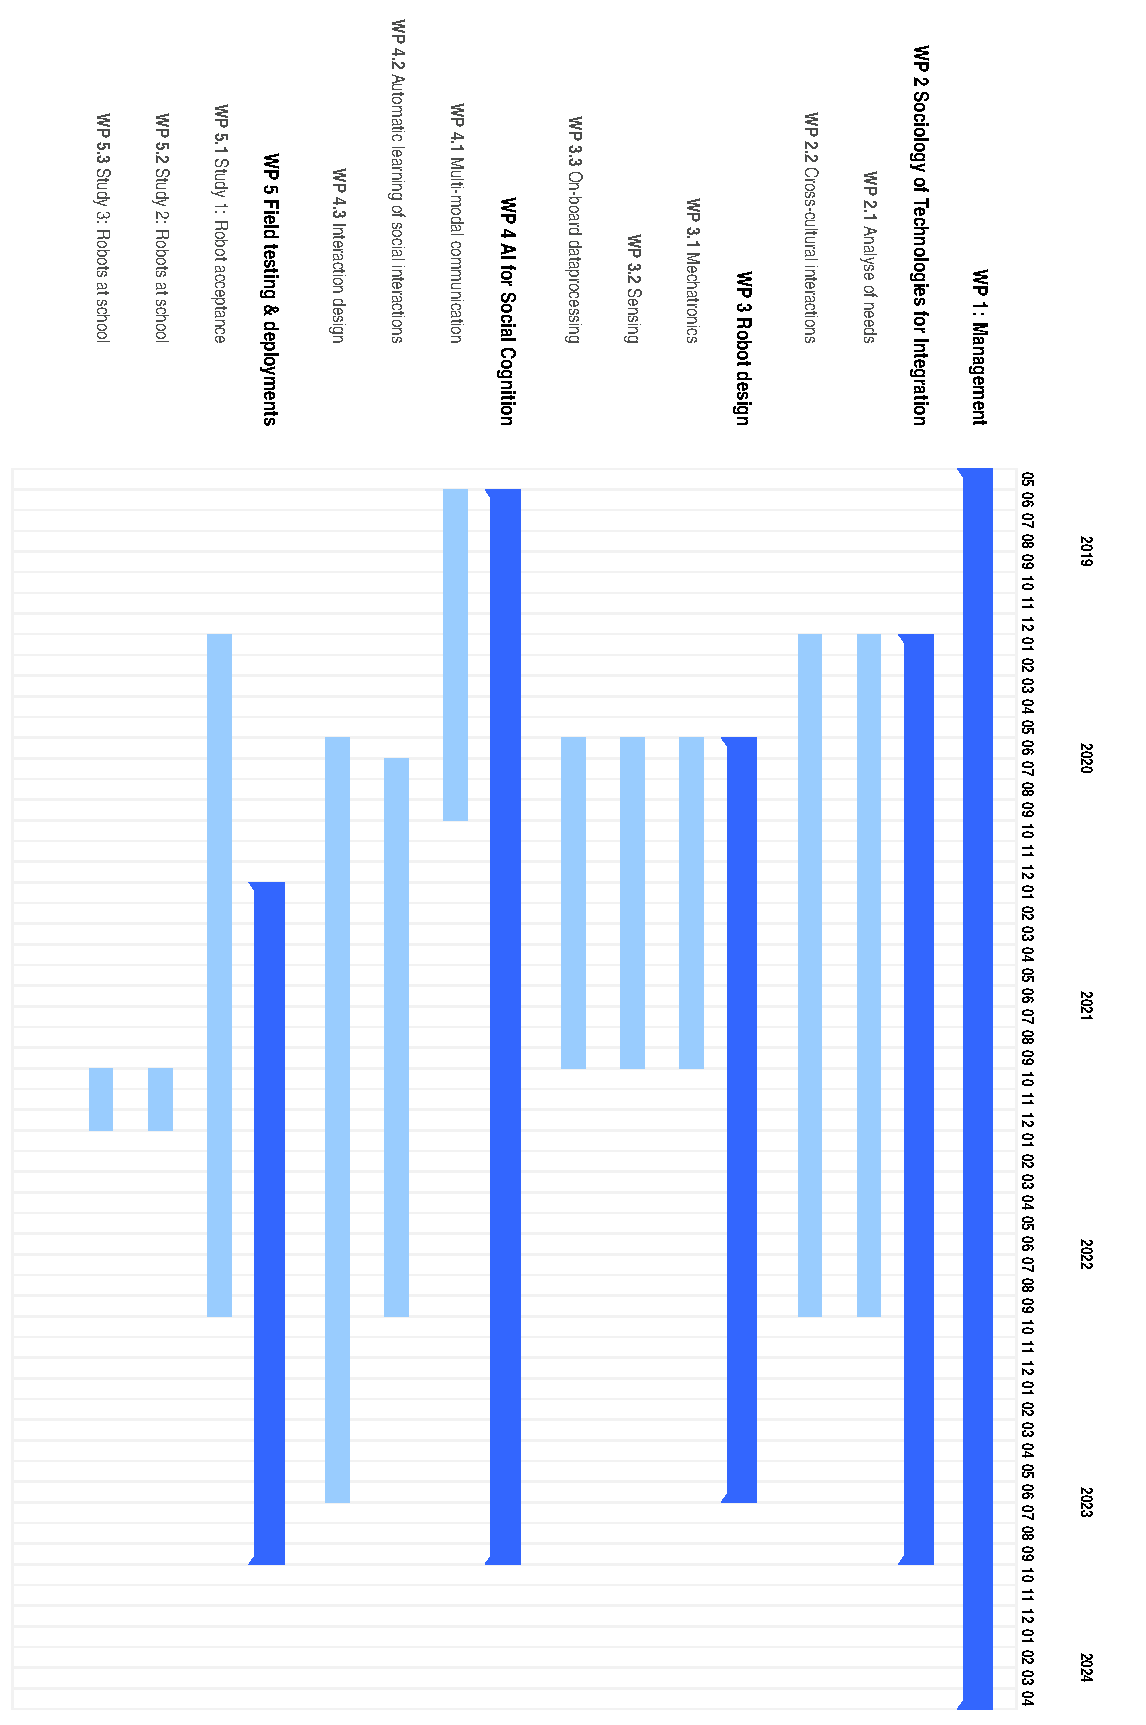
\includegraphics[width=\textwidth,height=25cm]{gantt.pdf}\\

\hypertarget{workpackage-interrelations}{%
\subsubsection{Workpackage
interrelations}\label{workpackage-interrelations}}

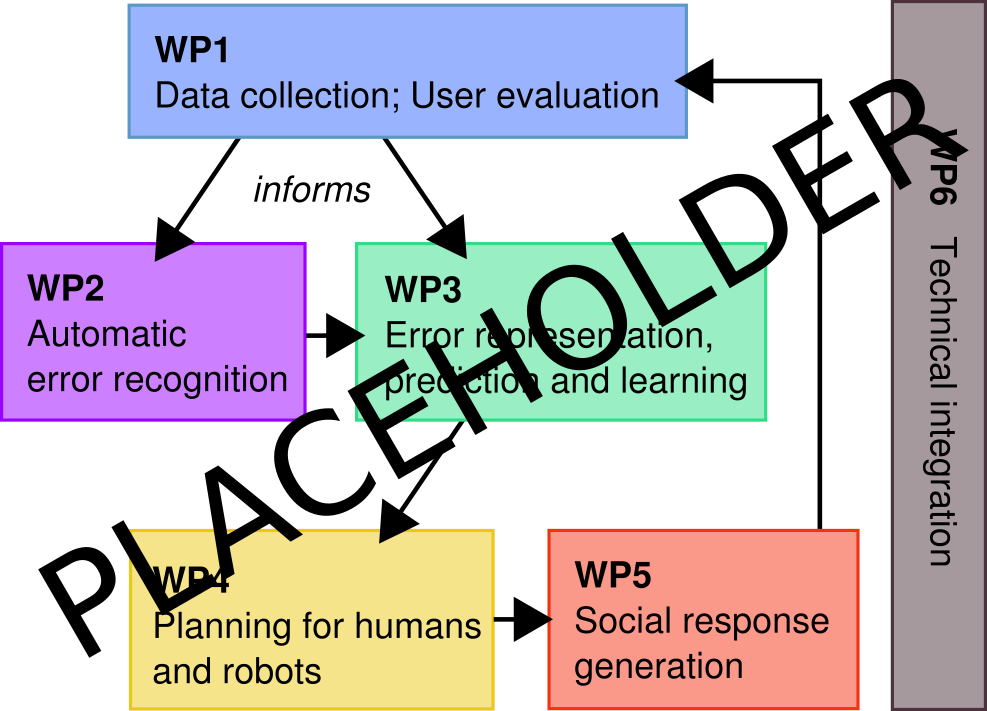
\includegraphics{figs/wp-interrelations.png}\\

\hypertarget{management-structure-milestones-and-procedures}{%
\subsection{Management structure, milestones and
procedures}\label{management-structure-milestones-and-procedures}}

\hypertarget{milestones}{%
\subsubsection{Milestones}\label{milestones}}

\begin{itemize}
\tightlist
\item
  week-long tests with local children in local schools
\item
  field deployment with one child in one school
\end{itemize}

\begin{longtable}[]{@{}lllll@{}}
\toprule
\begin{minipage}[b]{0.16\columnwidth}\raggedright
Milestone number\strut
\end{minipage} & \begin{minipage}[b]{0.14\columnwidth}\raggedright
Milestone name\strut
\end{minipage} & \begin{minipage}[b]{0.22\columnwidth}\raggedright
Related work package(s)\strut
\end{minipage} & \begin{minipage}[b]{0.14\columnwidth}\raggedright
Estimated date\strut
\end{minipage} & \begin{minipage}[b]{0.20\columnwidth}\raggedright
Means of verification\strut
\end{minipage}\tabularnewline
\midrule
\endhead
\begin{minipage}[t]{0.16\columnwidth}\raggedright
\strut
\end{minipage} & \begin{minipage}[t]{0.14\columnwidth}\raggedright
\strut
\end{minipage} & \begin{minipage}[t]{0.22\columnwidth}\raggedright
\strut
\end{minipage} & \begin{minipage}[t]{0.14\columnwidth}\raggedright
\strut
\end{minipage} & \begin{minipage}[t]{0.20\columnwidth}\raggedright
\strut
\end{minipage}\tabularnewline
\begin{minipage}[t]{0.16\columnwidth}\raggedright
\strut
\end{minipage} & \begin{minipage}[t]{0.14\columnwidth}\raggedright
\strut
\end{minipage} & \begin{minipage}[t]{0.22\columnwidth}\raggedright
\strut
\end{minipage} & \begin{minipage}[t]{0.14\columnwidth}\raggedright
\strut
\end{minipage} & \begin{minipage}[t]{0.20\columnwidth}\raggedright
\strut
\end{minipage}\tabularnewline
\begin{minipage}[t]{0.16\columnwidth}\raggedright
\strut
\end{minipage} & \begin{minipage}[t]{0.14\columnwidth}\raggedright
\strut
\end{minipage} & \begin{minipage}[t]{0.22\columnwidth}\raggedright
\strut
\end{minipage} & \begin{minipage}[t]{0.14\columnwidth}\raggedright
\strut
\end{minipage} & \begin{minipage}[t]{0.20\columnwidth}\raggedright
\strut
\end{minipage}\tabularnewline
\begin{minipage}[t]{0.16\columnwidth}\raggedright
\strut
\end{minipage} & \begin{minipage}[t]{0.14\columnwidth}\raggedright
\strut
\end{minipage} & \begin{minipage}[t]{0.22\columnwidth}\raggedright
\strut
\end{minipage} & \begin{minipage}[t]{0.14\columnwidth}\raggedright
\strut
\end{minipage} & \begin{minipage}[t]{0.20\columnwidth}\raggedright
\strut
\end{minipage}\tabularnewline
\bottomrule
\end{longtable}

\hypertarget{risks}{%
\subsubsection{Risks}\label{risks}}

\begin{longtable}[]{@{}lll@{}}
\toprule
\begin{minipage}[b]{0.26\columnwidth}\raggedright
Description of risk\strut
\end{minipage} & \begin{minipage}[b]{0.28\columnwidth}\raggedright
Work package(s) involved\strut
\end{minipage} & \begin{minipage}[b]{0.37\columnwidth}\raggedright
Proposed risk mitigation measures\strut
\end{minipage}\tabularnewline
\midrule
\endhead
\begin{minipage}[t]{0.26\columnwidth}\raggedright
risk 1 (low/medium/high)\strut
\end{minipage} & \begin{minipage}[t]{0.28\columnwidth}\raggedright
\strut
\end{minipage} & \begin{minipage}[t]{0.37\columnwidth}\raggedright
\strut
\end{minipage}\tabularnewline
\begin{minipage}[t]{0.26\columnwidth}\raggedright
\strut
\end{minipage} & \begin{minipage}[t]{0.28\columnwidth}\raggedright
\strut
\end{minipage} & \begin{minipage}[t]{0.37\columnwidth}\raggedright
\strut
\end{minipage}\tabularnewline
\begin{minipage}[t]{0.26\columnwidth}\raggedright
\strut
\end{minipage} & \begin{minipage}[t]{0.28\columnwidth}\raggedright
\strut
\end{minipage} & \begin{minipage}[t]{0.37\columnwidth}\raggedright
\strut
\end{minipage}\tabularnewline
\begin{minipage}[t]{0.26\columnwidth}\raggedright
\strut
\end{minipage} & \begin{minipage}[t]{0.28\columnwidth}\raggedright
\strut
\end{minipage} & \begin{minipage}[t]{0.37\columnwidth}\raggedright
\strut
\end{minipage}\tabularnewline
\bottomrule
\end{longtable}

\hypertarget{relevance-of-expertise-in-the-consortium}{%
\subsection{Relevance of expertise in the
consortium}\label{relevance-of-expertise-in-the-consortium}}

This project is ambitious, and brings together five leading groups in
social human-robot interaction, interaction design and human
socio-developmental psychology, with unique expertise and contributions:
The Bristol Robotics Lab, the largest UK robotic lab, has a long history
of running and leading complex projects involving hardware, software and
AI, with a strong track record in human-robot interaction and assistive
robotics; the University of Ghent will provide world-leading expertise
on robot design for interaction with children; the EPFL's CHILI lab has
a unique expertise in blending technology (and social robotics in
particular) in teaching environments, with a focus on rich social
interaction; the IST is recognised as a leading group in expressive
social agents and also has a very strong track record in child-robot
interactions; finally {[}socio-psychology partner{]}.

Critically, the complex interaction design that lies at the core of the
project will be informed and co-led by the Refugee Support department of
RedCross UK, one of the largest NGO world-wide.

\hypertarget{appropriate-allocation-and-justification-of-resources}{%
\subsection{Appropriate allocation and justification of
resources}\label{appropriate-allocation-and-justification-of-resources}}

(person-months, equipment, budget)

\textbf{Summary of staff effort}

\begin{longtable}[]{@{}llllllll@{}}
\toprule
& WP1 & WP2 & WP3 & WP4 & WP5 & WP6 & Total person/months per
participant\tabularnewline
\midrule
\endhead
BRL & & & & & & &\tabularnewline
GHE & & & & & & &\tabularnewline
EPFL & & & & & & &\tabularnewline
IST & & & & & & &\tabularnewline
RUN & & & & & & &\tabularnewline
RCUK & & & & & & &\tabularnewline
Total person/ month & & & & & & &\tabularnewline
\bottomrule
\end{longtable}

\textbf{Other direct cost}

\begin{longtable}[]{@{}lll@{}}
\toprule
BRL & Cost & Justification\tabularnewline
\midrule
\endhead
Travel & &\tabularnewline
Equipment & &\tabularnewline
Other goods and services & &\tabularnewline
Total & &\tabularnewline
\bottomrule
\end{longtable}

\newpage

\hypertarget{members-of-the-consortium}{%
\section{Members of the consortium}\label{members-of-the-consortium}}

\hypertarget{participants}{%
\subsection{Participants}\label{participants}}

For each partners:

\begin{itemize}
\tightlist
\item
  a description of the legal entity and its main tasks, with an
  explanation of how its profile matches the tasks in the proposal;
\item
  a curriculum vitae or description of the profile of the persons,
  including their gender, who will be primarily responsible for carrying
  out the proposed research and/or innovation activities;
\item
  a list of up to 5 relevant publications, and/or products, services
  (including widely-used datasets or software), or other achievements
  relevant to the call content;
\item
  a list of up to 5 relevant previous projects or activities, connected
  to the subject of this proposal;
\item
  a description of any significant infrastructure and/or any major items
  of technical equipment, relevant to the proposed work;
\end{itemize}

\hypertarget{bristol-robotics-lab}{%
\subsubsection{Bristol Robotics Lab}\label{bristol-robotics-lab}}

\hypertarget{institution}{%
\paragraph{Institution}\label{institution}}

The \emph{Bristol Robotics Laboratory (BRL)} is the largest co-located
and most comprehensive advanced robotics research establishment in the
UK. It is a joint venture between the University of the West of England
and the University of Bristol. BRL's multidisciplinary approach aims to
create autonomous devices capable of working independently, with each
other, or with humans. BRL draws on robotics, electrical \& mechanical
engineering, computer science, psychology, cognitive science and
sociology. BRL has an international reputation as a leading research
centre in advanced robotics research and has over 250 researchers
working on a broad portfolio of topics: HRI, collective robotics, aerial
robotics, neuro-inspired control, haptics, control systems, energy
harvesting and self-sustaining systems, rehabilitation robotics, soft
robotics and biomedical systems. BRL has many collaboration
partnerships, both national and international, and is experienced in
managing large multi-site projects. BRL has support from two embedded
units specialising in business and enterprise, together with an
incubator and successful track record of spin-outs.

\hypertarget{principal-investigators}{%
\paragraph{Principal investigators}\label{principal-investigators}}

Dr Séverin Lemaignan is Senior Researcher at the Bristol Robotics
Laboratory, University of the West of England, Bristol. Previously, he
obtained a joint PhD in Cognitive Robotics from the CNRS/LAAS (France)
and the Technical University of Munich (Germany) for which he received
the Best PhD in Robotics 2012 award from French CNRS. He then conducted
his research as Research Fellow at EPFL (Switzerland) and Plymouth
University (UK) where he was Lecturer in Robotics until 2018. Dr Séverin
Lemaignan has been involved in several European projects related to
social and cognitive robotics: CHRIS (Cooperative Human Robot
Interaction Systems), DREAM (Development of Robot-Enhanced therapy for
children with AutisM spectrum disorders), L2TOR (Second language
TutOring using social Robots). He has also been awarded in 2015 a EU
H2020 Marie Sklodowska-Curie Individual Fellowship for his project
DoRoThy (Donating Robots a Theory of Mind). His research interests
primarily concern the socio-cognitive aspects of human-robot
interaction, both from the perspective of the human cognition and the
design of cognitive architectures for the robots. More recently, he has
been focusing his experimental work on child-robot interactions in
educative settings, exploring how robots can support teachers and
therapists to develop effective and engaging novel learning paradigms.

Pr Manuel Giuliani\ldots{}

\hypertarget{university-of-ghent}{%
\subsubsection{University of Ghent}\label{university-of-ghent}}

\emph{Tony Belpaeme, Jelle Saldien}

\hypertarget{uxe9cole-polytechnique-fuxe9duxe9rale-de-lausanne}{%
\subsubsection{École Polytechnique Fédérale de
Lausanne}\label{uxe9cole-polytechnique-fuxe9duxe9rale-de-lausanne}}

\emph{Pierre Dillenbourg}

\hypertarget{instituto-superior-tuxe9cnico-university-of-lisbon}{%
\subsubsection{Instituto Superior Técnico, University of
Lisbon}\label{instituto-superior-tuxe9cnico-university-of-lisbon}}

\emph{Ana Paiva}

\hypertarget{academic-partner-in-sociology-radboud-university-nijmegen}{%
\subsubsection{Academic partner in sociology -- Radboud University
Nijmegen?}\label{academic-partner-in-sociology-radboud-university-nijmegen}}

\hypertarget{redcross-uk-rcuk}{%
\subsubsection{RedCross UK (RCUK)}\label{redcross-uk-rcuk}}

\emph{Alex Fraser}

\hypertarget{third-parties-involved-in-the-project}{%
\subsection{Third parties involved in the
project}\label{third-parties-involved-in-the-project}}

No third parties involved? maybe for some subcontracting?

\hypertarget{ethics-and-security}{%
\section{Ethics and Security}\label{ethics-and-security}}

\hypertarget{ethics}{%
\subsection{Ethics}\label{ethics}}

\hypertarget{security}{%
\subsection{Security}\label{security}}

\begin{itemize}
\tightlist
\item
  this project involves activities or results raising security issues:
  NO
\item
  this project involves `EU-classified information' as background or
  results: NO
\end{itemize}

\hypertarget{refs}{}
\leavevmode\hypertarget{ref-hostettler2016realtime}{}%
Hostettler, L., A. Özgür, S. Lemaignan, P. Dillenbourg, and F. Mondada.
2016. ``Real-Time High-Accuracy 2D Localization with Structured
Patterns.'' In \emph{Proceedings of the 2016 Ieee International
Conference on Robotics and Automation}.

\leavevmode\hypertarget{ref-ozgur2017cellulo}{}%
Özgür, A., S. Lemaignan, W. Johal, M. Beltran, M. Briod, L. Pereyre, F.
Mondada, and P. Dillenbourg. 2017. ``Cellulo: Versatile Handheld Robots
for Education.'' In \emph{Proceedings of the 2017 Acm/Ieee Human-Robot
Interaction Conference}. \url{https://doi.org/10.1145/2909824.3020247}.

\leavevmode\hypertarget{ref-ozgur2016permanent}{}%
Özgür, Ayberk, Wafa Johal, and Pierre Dillenbourg. 2016. ``Permanent
Magnet-Assisted Omnidirectional Ball Drive.'' In \emph{2016 Ieee/Rsj
International Conference on Intelligent Robots and Systems (Iros)},
1061--6. \url{https://doi.org/10.1109/IROS.2016.7759180}.

\end{document}
